\documentclass{standalone}

\usepackage{pgfplots}
\usepackage{pgfplotstable}

\pgfplotsset{compat=newest}

\begin{document}

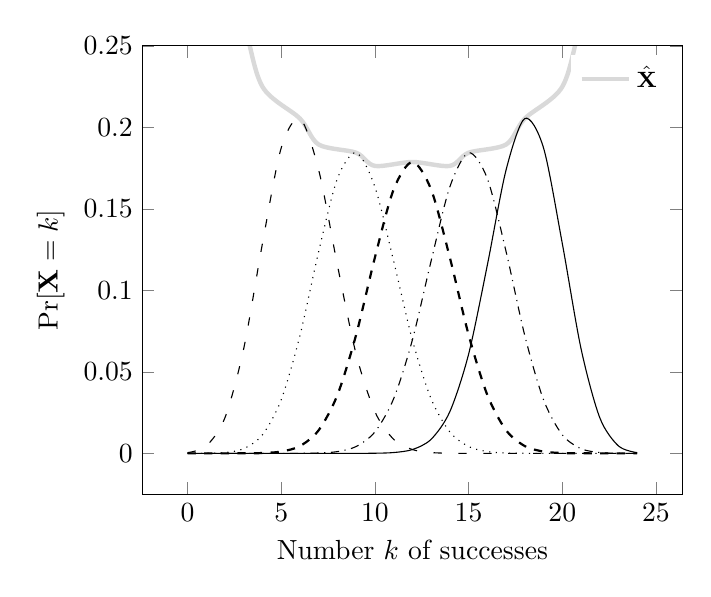
\begin{tikzpicture}[
  declare function = {
    binom(\n,\k) = \n! / (\k! * (\n - \k)!);
  },
  declare function = {
    hypergeom_dist_pmf(\N,\K,\n,\k)
      = binom(\K, \k) * binom(\N - \K, \n - \k) / binom(\N, \n);
  },
  declare function = {
    hypergeom_dist_mode(\N,\K,\n)
      = floor((\n + 1) * (\K + 1) / (\N + 2));
  },
]
  \def\samples{24}
  \pgfplotstableset{
    create on use/draws/.style = {
      create col/set list={0, 8, ..., 128}
    },
    create on use/modes/.style = {
      create col/expr = {
        hypergeom_dist_mode(128, \samples, \thisrow{draws})
      }
    },
    create on use/maxprob/.style = {
      create col/expr = {
        hypergeom_dist_pmf(128, \samples, \thisrow{draws}, \thisrow{modes})
      },
    },
  }

  \pgfplotstablenew[columns = {draws, modes, maxprob}]{\samples}{\loadedtable}

  \begin{axis}[
    samples at = {0, ..., \samples}, ymax = 0.25, smooth,
    ylabel = {$\Pr[\mathbf{X} = k]$}, xlabel = {Number $k$ of successes},
    legend style = { draw = none, font = \footnotesize, },
    yticklabel style = {
      /pgf/number format/fixed,
    },
  ]
    \addplot+[mark = none, solid, ultra thick, black, opacity = 0.15]
      table [x = modes, y = maxprob] {\loadedtable};
    \addlegendentry{$\hat{\mathbf{X}}$}

    \addplot+[black, loosely dashed, mark = none] {
      hypergeom_dist_pmf(128, \samples, 32, x)
    };

    \addplot+[black, dotted, mark = none] {
      hypergeom_dist_pmf(128, \samples, 48, x)
    };

    \addplot+[black, thick, dashed, mark = none] {
      hypergeom_dist_pmf(128, \samples, 64, x)
    };

    \addplot+[black, dashdotted, mark = none] {
      hypergeom_dist_pmf(128, \samples, 80, x)
    };

    \addplot+[black, solid, mark = none] {
      hypergeom_dist_pmf(128, \samples, 96, x)
    };
  \end{axis}
\end{tikzpicture}

\end{document}
